\subsection*{A gyakorlatokról}

\begin{center}
\begin{tabular}{l|cccc}
\toprule
\bf Kurzuskód	&\bf IB402-2&\bf IB402-3&\bf IB402-4	&\bf IB402-5\\
\midrule
\bf Időpont		& Sz 8-9		& Sz 9-10	& Sz 14-15		& Sz 15-16	\\
\bf Helyszín	& IR-223	&IR-223		& IR-223		& IR-223\\
\bottomrule
\end{tabular}
\end{center}

\begin{description}
\item[Gyakorlatvezető] Griechisch Erika
\item[Web] \url{http://www.inf.u-szeged.hu/~grerika}
\item[E-mail] \href{mailto:grerika@inf.u-szeged.hu}{grerika@inf.u-szeged.hu}
\item[Fogadóóra] Csütörtök 12-13
\item[Iroda] Árpád tér 2., II. emelet 221-es szoba
\item[Telefon] 62/54-3444 (csak belső hálózaton)
\end{description}


\subsection*{Követelmények}
\begin{center}
 \url{http://www.inf.u-szeged.hu/oktatas/kurzusleirasok/IB402.xml}
\end{center}



A vizsgára bocsátás feltétele a követelményekből minimum 20\% megszerzése (a maximális 50\%-ből). 
\bigskip

\begin{center}
\begin{tabular}{llr}
\toprule
			& \bf Időpont		& \%
			\\
			\midrule
Első kötprog 		&március 18. 23:59:59	& 5\\
Első zh 		&március 19-23		&15\\
Midterm 		&március 26-30		&10\\
Második kötprog 	&május 6 23:59:59	&5\\
Második zh 		&május 7-11		&15\\
\bottomrule
\end{tabular}
\end{center}
\bigskip

A fenti pontszerzési lehetőségek mással NEM pótolhatók, ezeken kívül más pontszerzési lehetőség nincs.
 
% Az elméleti vizsga két részből áll. Az első részben 10 kis kérdésre kell a hallgatóknak válaszolni, ahol összesen: 20\%-ot lehet szerezni. Majd 3 tételt (30\%) kapnak az előre kiadott tételjegyzékből. Az elméleti vizsgán összesen 50\%-ot lehet szerezni. Az elméleti vizsga akkor sikeres, ha a hallgató legalább 20\%-ot elér.
 

\bigskip

\begin{minipage}{0.5\textwidth}
\begin{description}
\item[0\%-49\%] 	elégtelen (1)
\item[50\%-61\%] 	elégséges (2)
\item[62\%-77\%] 	közepes (3)
\item[78\%-89\%] 	jó(4)
\item[90\%-100\%] 	jeles (5)
\end{description}
\end{minipage}

\subsection*{Hiányzás}
A laboratóriumi gyakorlatokon a részvétel kötelező, az egyes gyakorlatok pótlására nincs lehetőség.
%
 Az igazolás módja a foglalkozásokon és a vizsgán való távollét esetén {\color{red}{kizárólag}} hivatalos írásos igazolás fogadható el.



\subsection*{Ajánlott irodalmak}
\begin{minipage}{0.66\textwidth}
\begin{itemize}
\item \textsc{A.S. Tanenbaum:}\\
	\textit{Modern Operating Systems} (3rd Edition)
	%
\item \textsc{A.S. Tanenbaum, A.S. Woodhull:}\\
	\textit{Operációs rendszerek -- Tervezés és implementáció} (3. kiadás)
	%
\item \textsc{A.S. Tanenbaum:}\\ \textit{Distributed Operating Systems}
\end{itemize}
\end{minipage}
\begin{minipage}{0.33\textwidth}
\begin{flushright}

\includegraphics[height=3.5cm]{pics/TanenbaumMOS}
\hspace{2mm}
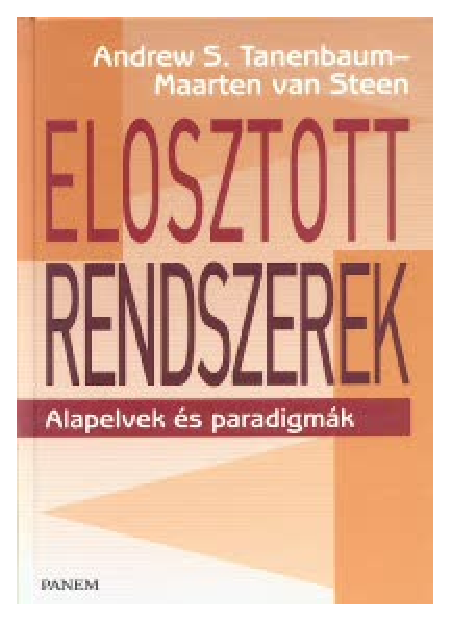
\includegraphics[height=3.5cm]{pics/TanenbaumDOS}
\end{flushright}
\end{minipage}


\subsection*{Ajánlott irodalom a gyakorlathoz}
\begin{itemize}
\item Rodek Lajos diasorozata a gyakorlathoz (a honlapomról elérhető)
\item Bevezetés a BASH programozásba\\ \url{http://tldp.fsf.hu/HOWTO/Bash-Prog-Intro-HOWTO-hu/Bash-Prog-Intro-HOWTO-hu.html}
\item \textsc{Büki András:} \textit{Héjprogramozás}\\ \url{http://www.kiskapu.hu/index.php?BODY=BookInfo&OP=details&ID=33247}
\item A GAWK felhasználói kézikönyv (letölthető!)\\ \url{http://hexahedron.hu/personal/peteri/gawk/index.html}
\end{itemize}

\subsection*{Linkek}
\subsubsection*{Linux}
\begin{itemize}
\item Általános: \url{http://www.linux.org/}, \url{http://www.linux.hu/}
\item Dokumentációk magyarul: \url{http://www.szabilinux.hu/index.html}
\item Fórum: \url{http://www.linuxempire.hu/}
\item Linux egyszerűen: \url{http://linuxegyszeruen.homelinux.org/}
\item Debian:
			\url{http://www.debian.org/}, 
			\url{http://www.aboutdebian.com/}
\item Ubuntu: 
			\url{http://www.ubuntu.com/},
			\url{http://ubuntu.hu/}%,
%			\url{http://women.ubuntu.hu/}
\end{itemize}

\subsubsection*{Gyakorlatvezetők weboldalai}
\begin{itemize}
\item \url{http://www.stud.u-szeged.hu/Najzer.Helga} (Najzer Helga)
\item \url{http://novakgabor.info} (Novák Gábor)
\item \url{http://www.stud.u-szeged.hu/Santa.Zsolt.1} (Sánta Zsolt)
\end{itemize}

\subsubsection*{Egyetem}
\begin{itemize}
\item \href{http://www.u-szeged.hu/}{Szegedi Tudományegyetem honlapja}
\item \href{https://www.etr.u-szeged.hu/}{SZTE Egységes Tanulmányi Rendszer}
\item \href{http://www.inf.u-szeged.hu}{SZTE Informatika Tanszékcsoport}
\end{itemize}

